\documentclass[a4paper]{article}
\usepackage{vntex}
\usepackage{enumitem}
\usepackage{float}
%\usepackage[english,vietnam]{babel}
%\usepackage[utf8]{inputenc}
\usepackage{mathptmx}[ptm]
%\usepackage[utf8]{inputenc}
%\usepackage[francais]{babel}
\usepackage{a4wide,amssymb,epsfig,latexsym,array,hhline,fancyhdr}
\usepackage[normalem]{ulem}
%\usepackage{soul}
\usepackage{pdfpages}
\usepackage[makeroom]{cancel}
\usepackage{amsmath}
\usepackage{amsthm}
\usepackage{multicol,longtable,amscd}
\usepackage{diagbox}%Make diagonal lines in tables
\usepackage{booktabs}
\usepackage{alltt}
\usepackage[framemethod=tikz]{mdframed}% For highlighting paragraph backgrounds
\usepackage{caption,subcaption}

\usepackage{lastpage}
\usepackage[lined,boxed,commentsnumbered]{algorithm2e}
\usepackage{enumerate}
\usepackage{color}
\usepackage{graphicx}							% Standard graphics package
\usepackage{array}
\usepackage{tabularx, caption}
\usepackage{multirow}
\usepackage{multicol}
\usepackage{rotating}
\usepackage{graphics}
\usepackage{geometry}
\usepackage{setspace}
\usepackage{epsfig}
\usepackage{tikz}

\usetikzlibrary{arrows,snakes,backgrounds,calc,positioning,shapes.geometric}
\usepackage[unicode]{hyperref}
\hypersetup{urlcolor=blue,linkcolor=black,citecolor=black,colorlinks=true} 
\usepackage{listings}

%\usepackage{pstcol} 								% PSTricks with the standard color package

\usepackage[normalem]{ulem}

\newtheorem{theorem}{{\bf Định lý}}
\newtheorem{property}{{\bf Tính chất}}
\newtheorem{proposition}{{\bf Mệnh đề}}
\newtheorem{corollary}[proposition]{{\bf Hệ quả}}
\newtheorem{lemma}[proposition]{{\bf Bổ đề}}
\theoremstyle{definition}
\newtheorem{exer}{Bài toán}

\def\thesislayout{	% A4: 210 × 297
	\geometry{
		a4paper,
		total={160mm,240mm},  % fix over page
		left=30mm,
		top=30mm,
	}
}
\def\thesisheadlayout{	% A4: 210 × 297
	\geometry{
		a4paper,
		total={160mm,240mm},  % fix over page
		left=30mm,
		top=10mm,
	}
}
\thesislayout
\lstset{
language=R,
basicstyle=\footnotesize\sffamily,
commentstyle=\ttfamily\color{black},
numbers=left,
numberstyle=\ttfamily\color{black}\footnotesize,
stepnumber=1,
numbersep=5pt,
backgroundcolor=\color{white},
showspaces=false,
showstringspaces=false,
showtabs=false,
frame=single,
tabsize=2,
captionpos=b,
breaklines=true,
breakatwhitespace=false,
title=\lstname,
escapeinside={},
keywordstyle={},
morekeywords={}
}
%\usepackage{fancyhdr}
\setlength{\headheight}{40pt}
\pagestyle{fancy}
\fancyhead{} % clear all header fields
\fancyhead[L]{
 \begin{tabular}{rl}
    \begin{picture}(25,15)(0,0)
    \put(0,-8){
\includegraphics[width=10mm, height=10mm]{Images/hcmut.png}}
    %\put(0,-8){
\epsfig{width=10mm,figure=hcmut.eps}}
   \end{picture}&
	%
\includegraphics[width=8mm, height=8mm]{hcmut.png} & %
	\begin{tabular}{l}
		\textbf{  Ho Chi Minh City University of Technology - VNUHCM }\\
		\textbf{  Faculty of Computer Science \& Engineering}
	\end{tabular} 	
 \end{tabular}
}
\fancyhead[R]{
	\begin{tabular}{l}
		\tiny \bf \\
		\tiny \bf 
	\end{tabular}  }
\fancyfoot{} % clear all footer fields
\fancyfoot[L]{\scriptsize  Internship Report (CO3335) - Semester 252, 2025 - 2026}
\fancyfoot[R]{\scriptsize  Page {\thepage}/\pageref{LastPage}}
\renewcommand{\headrulewidth}{0.3pt}
\renewcommand{\footrulewidth}{0.3pt}


%%%
\setcounter{secnumdepth}{4}
\setcounter{tocdepth}{4}
\makeatletter
\newcounter {subsubsubsection}[subsubsection]
\renewcommand\thesubsubsubsection{\thesubsubsection .\@alph\c@subsubsubsection}
\newcommand\subsubsubsection{\@startsection{subsubsubsection}{4}{\z@}%
                                     {-3.25ex\@plus -1ex \@minus -.2ex}%
                                     {1.5ex \@plus .2ex}%
                                     {\normalfont\normalsize\bfseries}}
\newcommand*\l@subsubsubsection{\@dottedtocline{3}{10.0em}{4.1em}}
\newcommand*{\subsubsubsectionmark}[1]{}
\makeatother

\everymath{\color{black}}%make in-line maths symbols blue to read/check easily

\sloppy
\captionsetup[figure]{labelfont={small,bf},textfont={small,it},belowskip=-1pt,aboveskip=-9pt,name=Image}
%space remove between caption, figure, and text
\captionsetup[table]{labelfont={small,bf},textfont={small,it},belowskip=-1pt,aboveskip=7pt,name=Images}
\setlength{\floatsep}{5pt plus 2pt minus 2pt}
\setlength{\textfloatsep}{5pt plus 2pt minus 2pt}
\setlength{\intextsep}{10pt plus 2pt minus 2pt}

\thesislayout

\begin{document}

\begin{titlepage}
\begin{tikzpicture}[remember picture, overlay]
  \draw[line width = 4pt] ($(current page.north west) + (0.4in,-0.5in)$) rectangle ($(current page.south east) + (-0.4in,0.5in)$);
  \draw[line width=1.5pt]
    ($ (current page.north west) + (0.45in,-0.55in) $)
    rectangle
    ($ (current page.south east) + (-0.45in,0.55in) $);
\end{tikzpicture}

\begin{center}
\Large \textbf{VIETNAM NATIONAL UNVIVERSITY, HO CHI MINH CITY} \\
\vspace{0.2cm}
\Large \textbf{HO CHI MINH CITY UNIVERSITY OF TECHNOLOGY} \\
\vspace{0.2cm}
\Large \textbf{FACULTY OF COMPUTER SCIENCE AND ENGINEERING}
\end{center}

\vspace{0.3cm}

\begin{figure}[h!]
\begin{center}

\includegraphics[width=4cm]{Images/hcmut.png}
\end{center}
\end{figure}

\begin{center}
\begin{tabular}{c}
\multicolumn{0}{c}{\textbf{{\LARGE INTERNSHIP REPORT}}}\\
\\
\\
\textbf{\Large SEMESTER 252 \- ACADEMIC YEAR 2025-2026} \\
\end{tabular}
\end{center}
\vspace{0.5cm}
\begin{itemize}
\renewcommand\labelitemi{--}
\item {\Large \bfseries MAJOR: \mdseries COMPUTER SCIENCE AND ENGINEERING}
\item {\Large \bfseries EDUCATION PROGRAM: \mdseries ENGLISH-TAUGHT PROGRAM}
\end{itemize}

\vspace{0.7cm}

\begin{itemize}
\renewcommand\labelitemi{--}
\item {\Large \bfseries INTERNSHIP ENTERPRISE:} {\Large \mdseries GreenNode Joint Stock Company}
\item {\Large \bfseries COMPANY SUPERVISOR: \mdseries \\ NGUYÊN DUY VŨ}
\item {\Large \bfseries FACULTY ADVISOR / SUPERVISOR / REPORT EVALUATOR:}\\
      {\Large \mdseries HOÀNG LÊ HẢI THANH}
\item {\Large \bfseries IMPLEMENTATION STUDENT (SVTH):}\\
      {\Large \bfseries FULL NAME: \mdseries NGUYỄN QUỐC HIỆU \quad \bfseries STUDENT ID: \mdseries 2352344}\\
\end{itemize}
\vspace{0.5cm}
\begin{center}
{\Large Ho Chi Minh City, August 2026}
\end{center}
\end{titlepage}


%\thispagestyle{empty}

\newpage
\renewcommand{\contentsname}{Contents} % hoặc "CONTENTS"
\tableofcontents
\newpage
\input{ChuongTrinhThucTap}
\section{Application Result}
% Insert hình kết quả của công ty bạn tại đây. Kết quả có thể được xem tại link \href{https://drive.google.com/drive/u/1/folders/1WY1-qFcrsiqiFtSjrSmL5bGh9wd1GulV}{này} (\textit{dùng mail HCMUT để truy cập})%
% \\ Đừng quên rằng báo cáo này sẽ được nộp kèm \href{https://drive.google.com/drive/u/1/folders/1KR1yhCCZYzp2QifAMwU5VtFU5_aP-F6y}{Form thăm dò sinh viên} (in riêng) nha mọi người.%

\begin{figure}[!h]
    \centering
    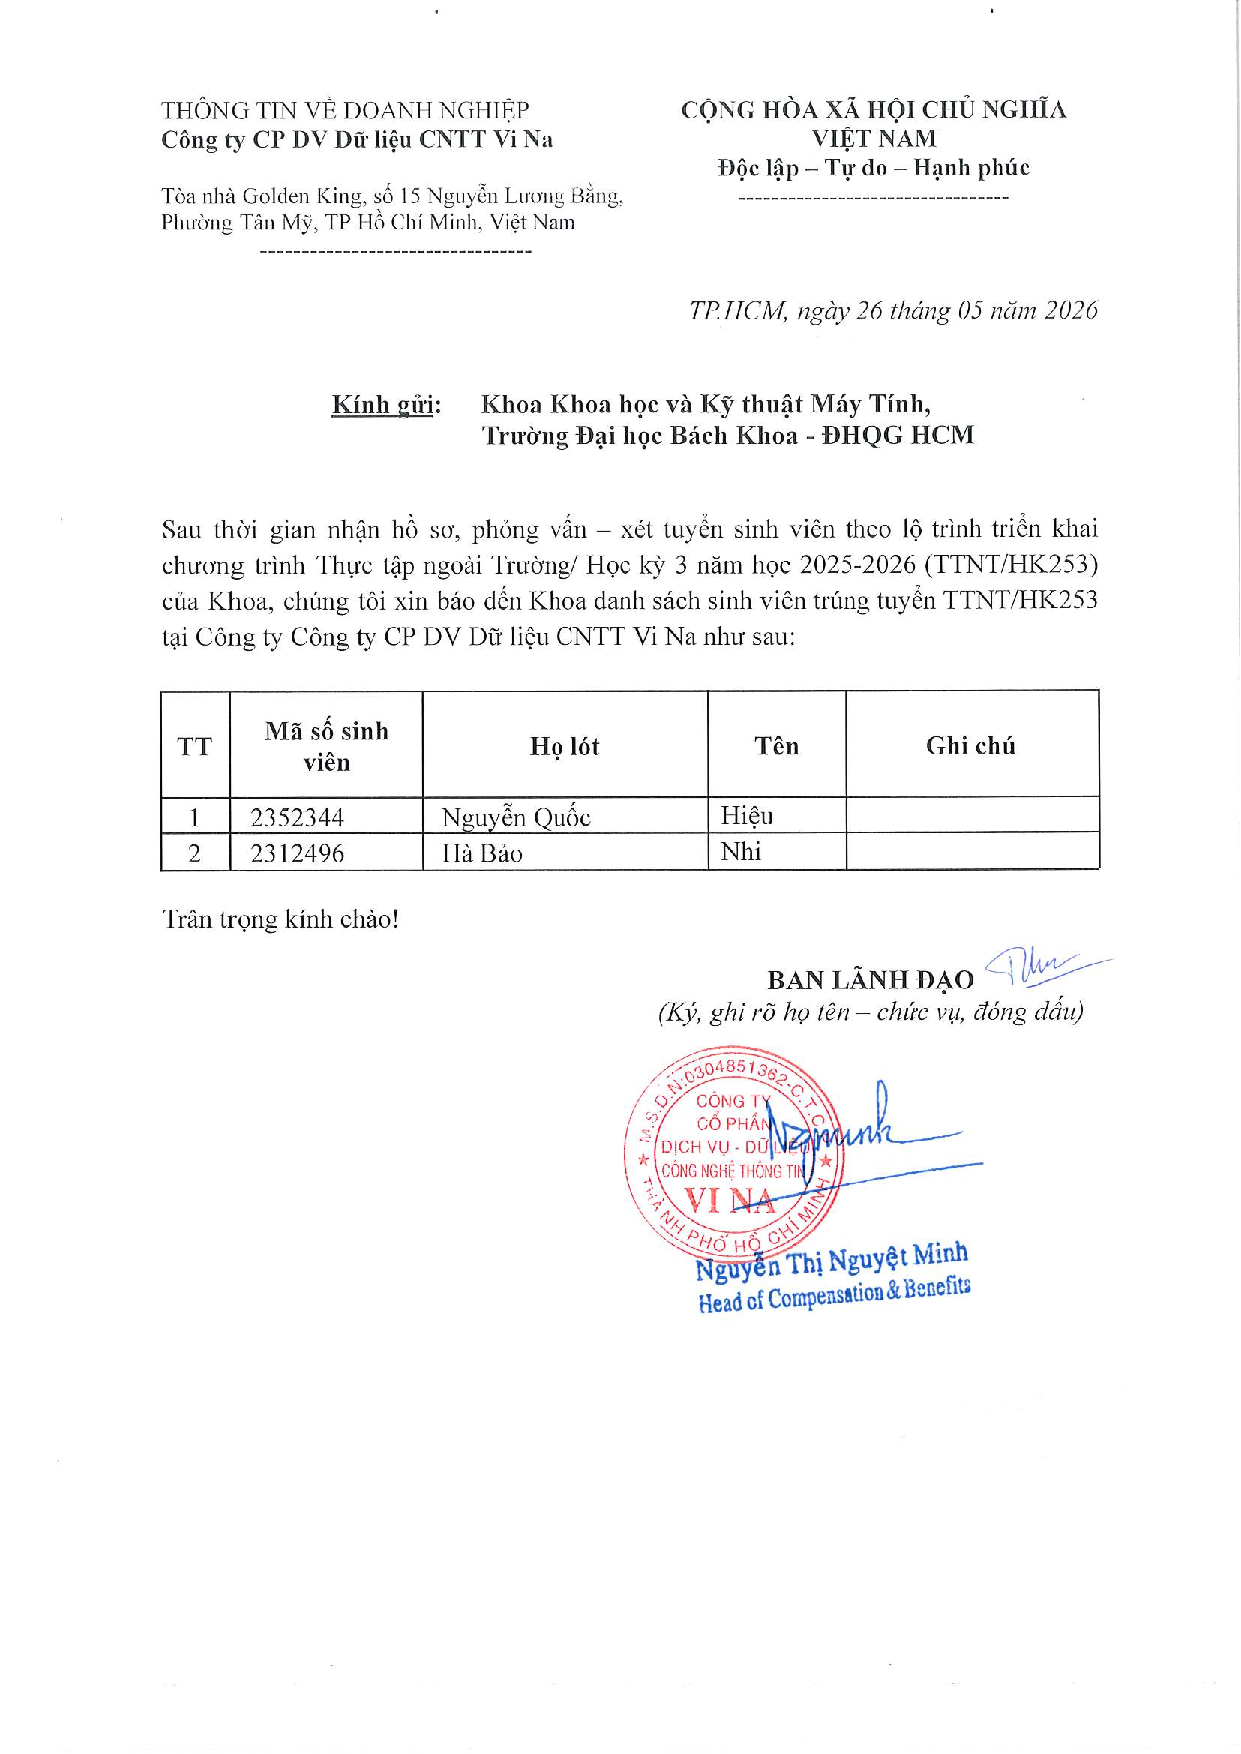
\includegraphics[width=1\linewidth]{Images/GIP_D3_TTNT_HK243.pdf}
    \caption{Kết quả xét tuyển công ty GIP}
    \label{fig:enter-label}
\end{figure}
\section{Internship Report}
% \subsection{Overview}

\subsection{Introduction to Greennode Corporation}

\subsubsection{General Information}

GreenNode is a Vietnam-based sovereign, high-performance AI cloud provider and a member of VNG Digital Business, under VNG Corporation, Vietnam's first technology unicorn, founded in 2004. In late 2025, VNG merged its cloud computing unit, VNG Cloud, with its AI infrastructure unit, GreenNode, into a single unified AI cloud brand, and this positioned it as one of the few platforms in Vietnam offering both conventional cloud and high-performance AI cloud on a unified ecosystem, letting customers train, fine-tune, and deploy AI models on the same infrastructure. As a preferred NVIDIA Cloud Service Partner in Southeast Asia, GreenNode offers enterprises high-performance NVIDIA H100 GPU infrastructure across data centers in Vietnam and Thailand, and it has supported over 1,000 domestic and international enterprises with a strong presence in markets such as the United States, MENA, and APAC, alongside active operations in Vietnam, Thailand, and Singapore. Its portfolio spans cloud infrastructure, AI/ML services, and data management and process-automation solutions, including PaaS offerings like vDB, Kafka, and VKS, as well as its in-house GreenNode IDP (Intelligent Document Processing) solution, which combines OCR, Generative AI, and LLMs to extract and validate data from complex documents.

\begin{figure}[!h]
    \centering
    
\includegraphics[width=0.5\linewidth]{Images/greennode.jpeg}
    \caption{Greennode company logo}
    \label{fig:logo}
\end{figure}

\subsubsection{Business Areas}

GreenNode focuses on the following main areas:
\begin{itemize}
    \item \textbf{AI Cloud Services:} The company's core business, providing sovereign, high-performance AI cloud infrastructure and enterprise AI/ML services, built on NVIDIA GPU infrastructure (H100), with platform services such as vDB, Kafka, and VKS, enabling customers to train, fine-tune, and deploy AI models.

    \item \textbf{Data Management and Automation:} Investment in developing solutions for data management, process automation, and intelligent document processing (e.g., GreenNode IDP, combining OCR, Generative AI, and LLMs to process unstructured documents).

    \item \textbf{Strategic Partnerships:} GreenNode is a preferred NVIDIA Cloud Service Partner (CSP) in Southeast Asia and has supported over 1,000 domestic and international enterprises across banking, insurance, securities, retail, and technology sectors.

    \item \textbf{International markets:} GreenNode operates data centers and services in Vietnam, Thailand, and Singapore, with an expanding customer presence in the United States, MENA, and APAC regions.
\end{itemize}

\subsubsection{Corporate Culture and Work Environment}

At GreenNode, corporate culture is not just a set of rules on paper but a source of inspiration for daily activities. The company encourages a creative and flexible working spirit, enabling individuals to proactively adapt to the fast-evolving AI and cloud computing landscape. Team spirit is considered the bond that unites all members, creating a strong collective working toward common goals.

Thanks to these core values, GreenNode's work environment is youthful, dynamic, and professional. Employees work in an open space where ideas are heard and respected. In addition to attractive benefits, the company emphasizes team-building and annual events, turning the workplace into a true "family," where everyone works with passion and enthusiasm.
\subsection{Internship Content}

\subsubsection{Objectives}

The internship topic is \emph{“AI Innovation for Internal Product Development.”} The goal is to build an AI-powered internal product that brings measurable value and drives adoption across the organization. This initiative aims to establish sustainable AI practices within the working environment and transform GreenNode into an AI-native organization, embedding intelligent automation and data-driven decision-making into core business processes and operational workflows.

\subsubsection{Detailed Weekly Tasks and Project Roadmap}

The three-month internship progressed from agent foundations and prototype development to SRE Agent implementation, supporting sandbox research, harness design, infrastructure analysis, and a Deep Agent migration proposal.

\subsubsubsection*{Phase 1: Agent Foundations and Prototype Development}
\phantomsection
\addcontentsline{toc}{subsubsubsection}{Phase 1: Agent Foundations and Prototype Development}

Month 1 established the foundations for building and evaluating the first agent prototype.

\subsubsubsection{Week 1: Onboarding and LLM Fundamentals}

During the first week, I joined the team, learned the development workflow, and prepared the local environment for the internship. I studied the role of large language models in agentic systems, focusing on prompting, context, reasoning, response generation, and interaction with external tools rather than low-level model architecture.

\subsubsubsection*{Task Description}

\begin{itemize}
    \item \textbf{Team Onboarding and Environment Setup}
    \begin{itemize}
        \item Attended initial orientation meeting with internship supervisor and team members.
        \item Learned team SOPs, development tools (Git, IDEs, CI/CD pipelines), communication channels, and code review processes.
        \item Aligned internship KPIs with supervisor: project scope, deliverables, and success criteria for the 3-month program.
        \item Set up development environment: cloned repositories, configured local development stack.
    \end{itemize}

    \item \textbf{LLMs as Components of AI Agents}
    \begin{itemize}
        \item Studied the role of LLMs as reasoning and decision-making components inside AI agents.
        \item Focused on prompts, context, task instructions, structured outputs, and interaction with external tools.
        \item Examined how an agent uses an LLM to interpret a request, plan actions, evaluate tool results, and produce a response.
        \item Reviewed practical agent applications such as research assistance, code-related tasks, operational support, and self-reflection.
    \end{itemize}
\end{itemize}

\subsubsubsection*{Results / Knowledge Gained}

\begin{itemize}
    \item Gained clear understanding of team workflows, tools, and expectations.
    \item Understood how LLMs support agent reasoning, planning, tool use, and response generation.
    \item Identified the importance of prompts, context, structured outputs, and clear tool interfaces in agent behavior.
    \item Established the foundation for subsequent agent framework and workflow development.
    \item Set clear project goals and alignment with supervisor for the internship period.
\end{itemize}

\subsubsubsection{Week 2: Agent Frameworks Exploration}

During the second week, I compared agent frameworks and studied the main patterns used to build agents. I focused on LangGraph, ReAct, reflection, self-critique, and tool use, then implemented small prototypes to observe state flow, callbacks, reflection behavior, and tool interaction before selecting a practical direction for the project.

\subsubsubsection*{Task Description}

\begin{itemize}
    \item \textbf{Established Weekly Meeting Cadence}
    \begin{itemize}
        \item Started regular weekly synchronization meetings with supervisor (typically 1-2 hours).
        \item Set meeting agenda: reviewing completed tasks, discussing blockers, planning next steps.
        \item Established communication protocols for urgent issues and weekly progress updates.
    \end{itemize}

    \item \textbf{Survey of Agent Frameworks}
    \begin{itemize}
        \item Studied LangGraph: workflow definition, state management, and node-based execution model.
        \item Explored ReAct pattern: reasoning + acting loop, how agents decompose tasks and call tools.
        \item Investigated reflection and self-critique patterns: how agents evaluate and improve their own outputs.
        \item Examined tool-use design: defining tool interfaces, argument validation, and error handling.
        \item Compared trade-offs: flexibility vs. simplicity, performance vs. developer experience.
    \end{itemize}

    \item \textbf{Proof-of-Concept Implementations}
    \begin{itemize}
        \item Built minimal prototypes with LangGraph to understand state flow and callbacks.
        \item Implemented a simple ReAct agent with a mock tool (e.g., simple calculator or search function).
        \item Tested reflection loop with temperature settings, prompt variations, and evaluation metrics.
    \end{itemize}
\end{itemize}

\subsubsubsection*{Results / Knowledge Gained}

\begin{itemize}
    \item Established effective communication with supervisor; weekly meetings became a key feedback mechanism.
    \item Compared major agent frameworks and understood their architectural strengths.
    \item Grasped ReAct, reflection, and tool-use design patterns and when each is appropriate.
    \item Built practical intuition through small prototype experiments.
    \item Ready to select a framework and proceed to deeper implementation.
\end{itemize}

\subsubsubsection{Week 3: Agent Framework Deep Dive and Design}

During the third week, I selected LangGraph because its modular graph structure provided control over agent execution and state management. I designed the basic agent architecture, defined its state and tool interfaces, and mapped the flow from planning to tool invocation, reflection, and response generation. 

\subsubsubsection*{Task Description}

\begin{itemize}
    \item \textbf{Framework Selection and Mastery}
    \begin{itemize}
        \item Chosed \textbf{LangGraph} framework based on project requirements and team preferences. Langgraph was selected for its flexibility, modularity, and support for complex agent workflows which we can intervent in the lower level execution and state management. 
        \item Studied advanced features: custom state types, multi-agent patterns, streaming, and error recovery.
        \item Read framework documentation and examined real-world example projects.
    \end{itemize}

    \begin{figure}[H]
    \centering
    
\includegraphics[width=0.4\linewidth]{Images/langgraph_logo.png}
    \caption{LangGraph Agent Framework}
    \label{fig:langgraph}
    \end{figure}

    \item \textbf{Agent Architecture Design}
    \begin{figure}[H]
\centering
\resizebox{\linewidth}{!}{%
\begin{tikzpicture}[
    node distance=7mm and 9mm,
    box/.style={draw, rounded corners, align=center, minimum height=9mm,
                text width=28mm, fill=blue!8},
    decision/.style={diamond, draw, align=center, aspect=2.1,
                     inner sep=1pt, text width=22mm, fill=orange!15},
    line/.style={->, >=stealth, thick},
    loop/.style={->, >=stealth, thick, dashed}
]
    \node[box] (input) {User Input};
    \node[box, right=of input] (state) {Initialize\\Agent State};
    \node[box, right=of state] (observe) {Observe\\Context};
    \node[box, right=of observe] (plan) {Plan and\\Reason with LLM};
    \node[decision, right=of plan] (decide) {Next action?};
    \node[box, below=of decide] (tool) {Invoke Tool};
    \node[box, left=of tool] (result) {Receive Tool\\Result};
    \node[box, left=of result] (reflect) {Evaluate and\\Reflect};
    \node[box, above=of decide] (final) {Generate\\Final Response};

    \draw[line] (input) -- (state);
    \draw[line] (state) -- (observe);
    \draw[line] (observe) -- (plan);
    \draw[line] (plan) -- (decide);
    \draw[line] (decide) -- node[right, font=\scriptsize] {complete} (final);
    \draw[line] (decide) -- node[right, font=\scriptsize] {tool required} (tool);
    \draw[line] (tool) -- (result);
    \draw[line] (result) -- (reflect);
    \draw[loop]
        (reflect.north)
        -- node[right, fill=white, inner sep=1pt, font=\scriptsize]
        {continue}
        (observe.south);
\end{tikzpicture}%
}
\vspace{1pt}
\caption{Basic Agent Logic: State Initialization, Reasoning, Tool Use, and Reflection}
\label{fig:agent_logic}
\end{figure}
    \begin{itemize}
        \item Designed a basic two-capability agent:
        \begin{itemize}
            \item \textbf{Research capability:} gather information, search knowledge bases, retrieve documents.
            \item \textbf{Self-reflection capability:} evaluate outputs, identify weaknesses, generate improvement suggestions.
        \end{itemize}
        \item Defined state structure: input, intermediate thoughts, tool calls, results, final response.
        \item Mapped out the execution flow: planning $\rightarrow$ tool invocation $\rightarrow$ reflection $\rightarrow$ output.
        \item Designed tool interfaces: research (query), knowledge store (retrieve), and reflection (evaluate).
    \end{itemize}
\end{itemize}



\subsubsubsection*{Results / Knowledge Gained}

\begin{itemize}
    \item Achieved proficiency with chosen framework; understood advanced patterns.
    \item Created a solid architectural design for the basic agent with clear responsibilities.
    \item Defined data flow and state management approach suitable for complex agent behavior.
    \item Established clear implementation roadmap for the following week.
\end{itemize}

\subsubsubsection{Week 4: Basic Agent Implementation and Month 1 Review}

During the fourth week, I implemented the basic research and self-reflection agent from the design prepared in Week 3. I connected the agent loop, tested representative inputs, handled tool failures, evaluated response quality and latency, and presented the working prototype during the Month 1 review.

\subsubsubsection*{Task Description}

\begin{itemize}
    \item \textbf{Build and Refine Basic Agent}
    \begin{itemize}
        \item Implemented research capability: querying knowledge base, retrieving relevant documents, summarizing findings.
        \item Implemented self-reflection capability: analyzing response quality, identifying gaps, suggesting improvements.
        \item Built the complete agent loop: initialized state, executed planning, invoked tools, reflected on results.
        \item Tested end-to-end flow with sample inputs; fixed bugs and refined logic.
        \item Implemented error handling: graceful degradation when tools fail, retry logic.
    \end{itemize}

    \item \textbf{Agent Evaluation}
    \begin{itemize}
        \item Tested reflection loop quality: how well the agent identifies and corrects its own mistakes.
        \item Measured response latency and identify bottlenecks.
        \item Evaluated response quality: accuracy, relevance, and completeness of agent outputs.
    \end{itemize}

    \item \textbf{Month 1 Review with Supervisor}
    \begin{itemize}
        \item Presented working basic agent with demo.
        \item Discussed progress, challenges encountered, and lessons learned.
        \item Reviewed feedback and adjusted scope for Month 2 if needed.
        \item Confirmed readiness to proceed to sandbox integration phase.
    \end{itemize}
\end{itemize}

\subsubsubsection*{Results / Knowledge Gained}

\begin{itemize}
    \item Successfully built a functioning agent with research and self-reflection capabilities.
    \item Understood real-world considerations: error handling, performance, and robustness.
    \item Learned how reflection loops work in practice: when they help and when they may not.
    \item Received supervisor feedback and adjusted priorities for next phase.
    \item Completed Month 1 with a solid foundation for sandbox integration.
\end{itemize}

\newpage

\subsubsubsection*{Phase 2: SRE Agent Development and Sandbox Support}
\phantomsection
\addcontentsline{toc}{subsubsubsection}{Phase 2: SRE Agent Development and Sandbox Support}

Month 2 focused on building the SRE Agent and investigating sandboxing as a supporting execution capability.

\subsubsubsection{Week 5: SRE Agent Foundations and Operational Motivation}

During Week 5, I started building the SRE Agent from the agent foundations completed in Month 1. The agent was needed to support GreenNode's internal operations by turning operational requests into structured diagnostic workflows. Instead of relying on manual investigation across infrastructure components, the SRE Agent could interpret an incident request, plan diagnostic steps, invoke the appropriate tools, and evaluate the collected results in a consistent process.

\subsubsubsection*{Task Description}

\begin{itemize}
    \item \textbf{Motivation for Building the SRE Agent}
    \begin{itemize}
        \item Analyzed the need for an agent specialized in supporting internal Site Reliability Engineering tasks.
        \item Identified that operational troubleshooting requires coordinated reasoning across incident requests, diagnostic procedures, tools, and technical results.
        \item Defined the SRE Agent as a way to make these workflows more systematic, repeatable, and easier to extend.
    \end{itemize}

    \item \textbf{SRE Agent Initial Development}
    \begin{itemize}
        \item Built the initial SRE Agent from the agent foundations developed during Month 1.
        \item Defined the initial operational workflow: receiving an incident request, planning diagnostic steps, invoking tools, and reviewing results.
        \item Studied the required state, tool interfaces, and execution flow for an SRE-oriented agent.
        \item Set up the local development environment and established a baseline for later harness and infrastructure work.
    \end{itemize}
\end{itemize}

\subsubsubsection*{Results / Knowledge Gained}

\begin{itemize}
    \item Established the motivation, initial architecture, and execution flow of the SRE Agent.
    \item Connected agent reasoning and tool orchestration to concrete internal SRE troubleshooting needs.
    \item Prepared a clear baseline for continuing backend logic development in the following weeks.
\end{itemize}

\subsubsubsection{Week 6: SRE Agent Core Logic and Runtime Research}

During Week 6, I implemented and refined the SRE Agent backend logic. I worked on request interpretation, planning, state transitions, tool invocation, result evaluation, and error handling. After the core flow was established, I added Jaeger-based observability to trace LLM calls, tool invocations, decision loops, and execution latency. I also documented the execution requirements that would later guide the sandbox research and staging integration in Weeks 7--8.

\subsubsubsection*{Task Description}

\begin{itemize}
    \item \textbf{SRE Agent Core Logic}
    \begin{itemize}
        \item Implemented and refined the initial agent loop: request interpretation, planning, tool invocation, and result evaluation.
        \item Studied state management and error-handling requirements for operational workflows.
        \item Tested representative diagnostic flows and documented execution behavior.
    \end{itemize}

    \item \textbf{SRE Agent Observability and Monitoring}
    \begin{itemize}
        \item Studied Jaeger for tracing the SRE Agent's execution and decision flow after the core backend logic was established.
        \item Instrumented LLM calls, tool invocations, state transitions, and decision loops to analyze agent behavior.
        \item Observed decision latency, reasoning steps, reflection cycles, token usage, model latency, and tool performance.
        \item Used traces to identify execution bottlenecks, verify error handling, and improve the SRE Agent's operational workflow.
        \item Improved visibility into agent behavior and supported more transparent debugging of the backend logic.
    \end{itemize}

    \begin{figure}[!h]
    \centering
    
\includegraphics[width=0.35\linewidth]{Images/Jaeger_logo.png}
    \caption{Jaeger Distributed Tracing for SRE Agent Behavior}
    \label{fig:jaeger}
    \end{figure}

    \item \textbf{Execution Requirements for the Next Phase}
    \begin{itemize}
        \item Documented the execution, error-handling, and observability requirements for running agent tools safely.
        \item Prepared criteria for evaluating sandbox runtimes during the staging-environment integration in Weeks 7--8.
    \end{itemize}

    \begin{figure}[H]
        \centering

        \resizebox{0.9\linewidth}{!}{%
        \begin{tikzpicture}[
            node distance=12mm and 16mm,
            arch/.style={
                draw,
                rounded corners,
                align=center,
                minimum height=11mm,
                text width=38mm,
                fill=blue!8
            },
            graph/.style={
                draw,
                rounded corners,
                align=center,
                minimum height=17mm,
                text width=48mm,
                fill=blue!18,
                very thick
            },
            flow/.style={->, >=stealth, thick},
            trace/.style={->, >=stealth, thick, dashed}
        ]

            \node[arch] (request) {Operational\\Request};

            \node[graph, right=of request] (runtime) {
                Graph Runtime\\
                SRE Agent Logic\\
                \scriptsize
                interpret $\rightarrow$ plan $\rightarrow$
                invoke $\rightarrow$ evaluate
            };

            \node[arch, right=22mm of runtime, yshift=14mm]
                (observability) {Observability\\Jaeger Tracing};

            \node[arch, right=22mm of runtime, yshift=-14mm]
                (execution) {Sandbox};

            \draw[flow]
                (request.east) -- (runtime.west);

            \draw[trace]
                (runtime.north east)
                -- node[above, sloped, font=\scriptsize] {agent traces}
                (observability.west);

            \draw[flow]
                (runtime.south east)
                -- node[below, sloped, font=\scriptsize] {tool execution}
                (execution.west);

            \draw[flow, rounded corners]
                (execution.south)
                -- ++(0,-6mm)
                -| node[below, font=\scriptsize, pos=0.25] {results}
                (runtime.south);

        \end{tikzpicture}%
        }

        \vspace{4mm}

        \caption{SRE Agent Architecture}
        \label{fig:sre_architecture}
    \end{figure}
\end{itemize}

\subsubsubsection*{Results / Knowledge Gained}

\begin{itemize}
    \item Strengthened the SRE Agent's initial execution and tool-invocation logic.
    \item Produced runtime-selection criteria for the agent's future sandbox capability.
    \item Linked runtime research to concrete SRE Agent execution requirements.
\end{itemize}

\subsubsubsection{Week 7--8: Sandbox Research and SRE Agent Staging Integration}

During Weeks 7--8, I began researching sandboxing as a supporting execution environment for the SRE Agent and integrated it in the staging environment. The goal was to allow code-related or diagnostic actions to run with controlled isolation while keeping the SRE Agent's operational workflow unchanged. I continued refining the agent's diagnostic flow, tested staging execution paths and failure cases, and evaluated the runtime behavior of sandboxed actions.

\subsubsubsection*{Task Description}

\begin{itemize}
    \item \textbf{SRE Agent Development}
    \begin{itemize}
        \item Continued developing the SRE Agent's diagnostic workflow and tool integration.
        \item Traced execution paths, tested failure cases, and refined state transitions.
        \item Prepared the agent structure for controlled execution and later infrastructure-aware operations.
    \end{itemize}

    \item \textbf{Sandbox Research}
    \begin{itemize}
        \item Studied OpenSandbox and the security requirements for executing agent-generated or untrusted code.
        \item Compared runsc (gVisor), kata-fc (Firecracker), and kata-qemu (QEMU) according to isolation, startup latency, execution latency, memory footprint, and network throughput.
        \item Analyzed Kubernetes orchestration, resource limits, timeout handling, output capture, and cleanup requirements.
    \end{itemize}

    \item \textbf{Staging-Environment Integration}
    \begin{itemize}
        \item Integrated sandbox execution with the SRE Agent's tool-invocation path in the staging environment.
        \item Tested pod creation, code execution, output collection, cleanup, resource limits, and timeout handling.
        \item Verified the interaction between the SRE Agent backend logic and the sandbox without treating sandboxing as a separate project.
    \end{itemize}

    \item \textbf{Month 2 Review with Supervisor}
    \begin{itemize}
        \item Demonstrated the SRE Agent workflow and its supporting sandbox integration in staging.
        \item Presented the runtime research and explained how sandboxing supports safer agent operations.
        \item Reviewed the next phase: harness development, infrastructure research, and production-oriented design.
    \end{itemize}
\end{itemize}

\subsubsubsection*{Results / Knowledge Gained}

\begin{itemize}
    \item Advanced the SRE Agent from an initial workflow toward an infrastructure-aware operational agent.
    \item Gained practical knowledge of sandbox runtimes and integrated controlled execution into the SRE Agent staging environment.
    \item Established the foundation for Month 3 harness, governance, and infrastructure work.
\end{itemize}

\subsubsubsection{Week 9: SRE Agent Development and Architecture Review}

During Week 9, I continued developing the SRE Agent and reviewed its architecture as the project moved toward harness-oriented design. I traced how operational requests moved through state management, planning, tool integration, orchestration, and result evaluation. I also read the current source code and design documents to identify integration points and unresolved issues for the next phase.

\subsubsubsection*{Task Description}

\begin{itemize}
    \item \textbf{SRE Agent Architecture Development}
    \begin{itemize}
        \item Continued developing the SRE Agent architecture from the foundations established in Month 2.
        \item Integrated internal databases into the SRE Agent as tools for checking operational logs and diagnosing resource-related issues.
        \item Defined the main state-management, tool-integration, and orchestration responsibilities.
    \end{itemize}

    \item \textbf{Codebase and Design Review}
    \begin{itemize}
        \item Reviewed the current source code, architecture documents, and design decisions.
        \item Traced representative execution paths and identified integration points for the harness mechanism.
        \item Discussed design choices and current challenges with the mentor and team.
    \end{itemize}
\end{itemize}

\begin{figure}[H]
    \centering
    \begin{minipage}[b]{0.49\textwidth}
        \centering
        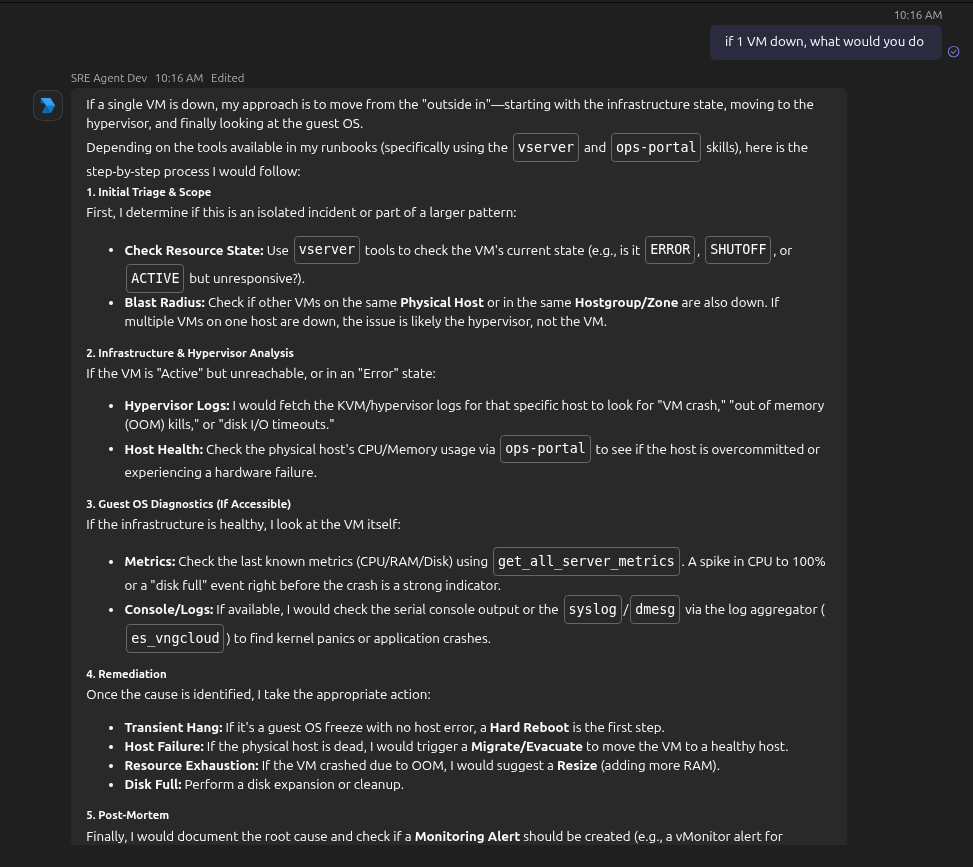
\includegraphics[width=\textwidth]{Images/demo_1.png}%
    \end{minipage}
    \hfill
    \begin{minipage}[b]{0.49\textwidth}
        \centering
        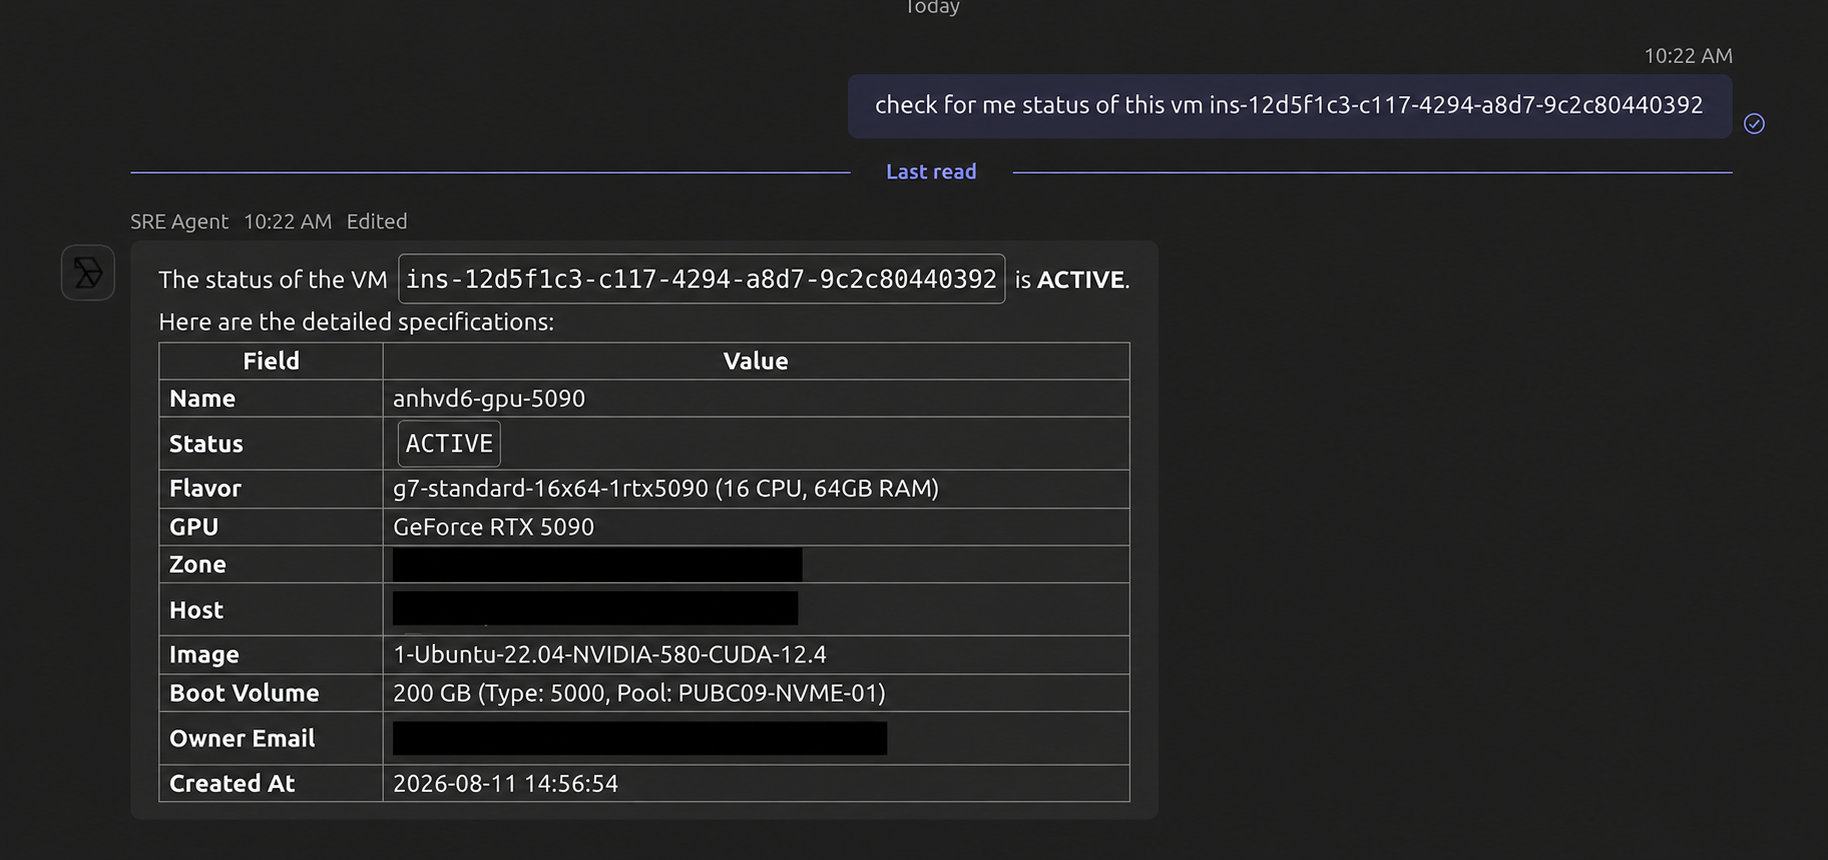
\includegraphics[width=\textwidth]{Images/demo_2.png}%
    \end{minipage}
    \vspace{10pt}
    \caption{Demo of SRE-Agent}
    \label{fig:sre_agent_demo}
\end{figure}

\subsubsubsection*{Results / Knowledge Gained}

\begin{itemize}
    \item Built a clear understanding of the SRE Agent architecture and its development direction.
    \item Connected the Month 2 agent workflow with the Month 3 harness and infrastructure tasks.
    \item Identified areas requiring deeper analysis and refinement.
\end{itemize}

\newpage

\subsubsubsection*{Phase 3: Harness Research, Deep Agent Seminar, and Migration Review}
\phantomsection
\addcontentsline{toc}{subsubsubsection}{Phase 3: Harness Research, Deep Agent Seminar, and Migration Review}

Month 3 focused on the scalability limitations of the LangGraph-based SRE Agent, research into the LangChain Deep Agent harness, knowledge sharing with the team, and preparation of a migration plan for review with the line manager.

\subsubsubsection{Week 10: LangGraph Scalability Review and Deep Agent Harness Research}

During Week 10, I investigated why the SRE Agent became difficult to scale as its LangGraph workflow grew. The increasing number of state transitions, tool integrations, execution controls, and operational requirements made the low-level graph implementation harder to extend and maintain. After surveying alternative approaches, I focused on the LangChain Deep Agent suite as a higher-level harness for improving the SRE Agent's stability, scalability, and developer experience.

\subsubsubsection*{Task Description}

\begin{itemize}
    \item \textbf{Analysis of the Existing LangGraph SRE Agent}
    \begin{itemize}
        \item Reviewed the current SRE Agent graph, state structure, nodes, tool interfaces, and execution transitions.
        \item Identified scaling difficulties caused by growing workflow complexity, duplicated control logic, and tightly coupled state and tool management.
        \item Recorded requirements for a higher-level harness, including context management, memory, loop control, observability, error handling, and controlled execution.
    \end{itemize}

    \item \textbf{Deep Research on the LangChain Deep Agent Harness}
    \begin{itemize}
        \item Studied the Deep Agent architecture, orchestration model, context and memory management, tool-use model, and execution lifecycle.
        \item Compared responsibilities handled explicitly in the LangGraph implementation with capabilities provided by the higher-level harness.
        \item Evaluated support for iteration limits, timeout handling, state persistence, tracing, human approval, permissions, and future multi-agent coordination.
        \item Mapped the existing SRE Agent tools and graph logic to potential Deep Agent integration points and identified migration constraints.
    \end{itemize}

    \item \textbf{Migration Architecture Design}
    \begin{itemize}
        \item Designed a migration direction in which existing SRE Agent capabilities remain the functional core while the Deep Agent harness manages orchestration and runtime concerns.
        \item Defined connections to Jaeger observability, the staging execution runtime, existing data-source tools, and future governance controls.
    \end{itemize}
\end{itemize}

\begin{figure}[H]
\centering
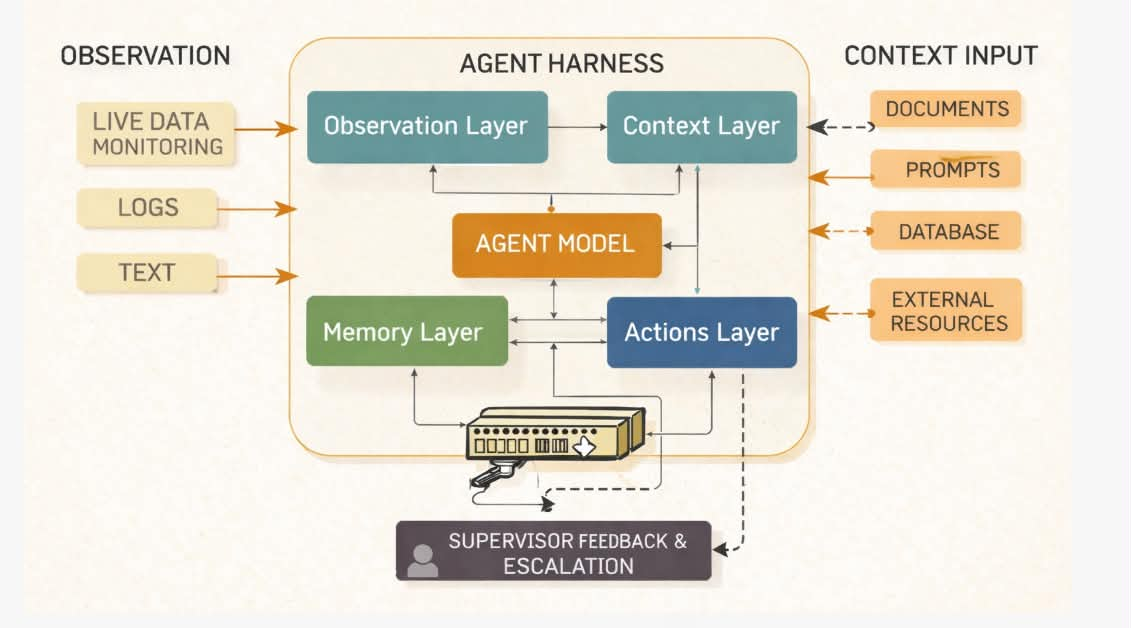
\includegraphics[width=0.9\linewidth]{Images/agent_harness_architecture.jpeg}
\caption{Agent Harness Architecture: Observation, Context, Model, Memory, and Actions Layers}
\label{fig:agent_harness}
\end{figure}

\subsubsubsection*{Results / Knowledge Gained}

\begin{itemize}
    \item Identified the main scalability and maintainability limitations of the LangGraph-based SRE Agent.
    \item Gained a detailed understanding of the LangChain Deep Agent harness and its relevance to the SRE workflow.
    \item Produced an initial migration architecture connecting existing SRE capabilities to the higher-level harness.
\end{itemize}

\subsubsubsection{Week 11: Deep Agent Seminar and Team Knowledge Sharing}

During Week 11, I transformed the Week 10 research into an internal seminar for the R\&D and engineering teams. The seminar explained the SRE Agent's current LangGraph architecture, the scaling problems observed during development, and how the LangChain Deep Agent harness could provide a more stable and scalable direction. I presented the technical comparison, migration concept, and expected impact on future SRE Agent development.

\subsubsubsection*{Task Description}

\begin{itemize}
    \item \textbf{Seminar Preparation}
    \begin{itemize}
        \item Organized the three-month development journey from agent foundations to SRE Agent implementation and harness research.
        \item Prepared diagrams explaining the current graph-runtime SRE Agent, the harness boundary, observability, and the planned execution runtime.
        \item Summarized the differences between the current LangGraph implementation and the LangChain Deep Agent approach.
    \end{itemize}

    \item \textbf{Internal Deep Agent Seminar}
    \begin{itemize}
        \item Delivered the seminar to the R\&D and engineering teams.
        \item Explained why the existing SRE Agent became difficult to scale and why a higher-level harness was considered.
        \item Presented Deep Agent architecture, orchestration, context and memory management, tool calling, observability, governance, and scalability considerations.
        \item Discussed how the proposed harness could preserve existing SRE Agent capabilities while reducing orchestration complexity.
        \item Conducted a question-and-answer session and collected technical feedback from the team.
    \end{itemize}

    \begin{figure}[H]
    \centering
    
\includegraphics[width=0.35\linewidth]{Images/deepagent_logo.png}
    \vspace{10pt}
    \caption{Deep Agent Framework}
    \label{fig:deepagent}
    \end{figure}

    \begin{figure}[H]
    \centering
    \begin{minipage}[b]{0.49\textwidth}
        \centering
        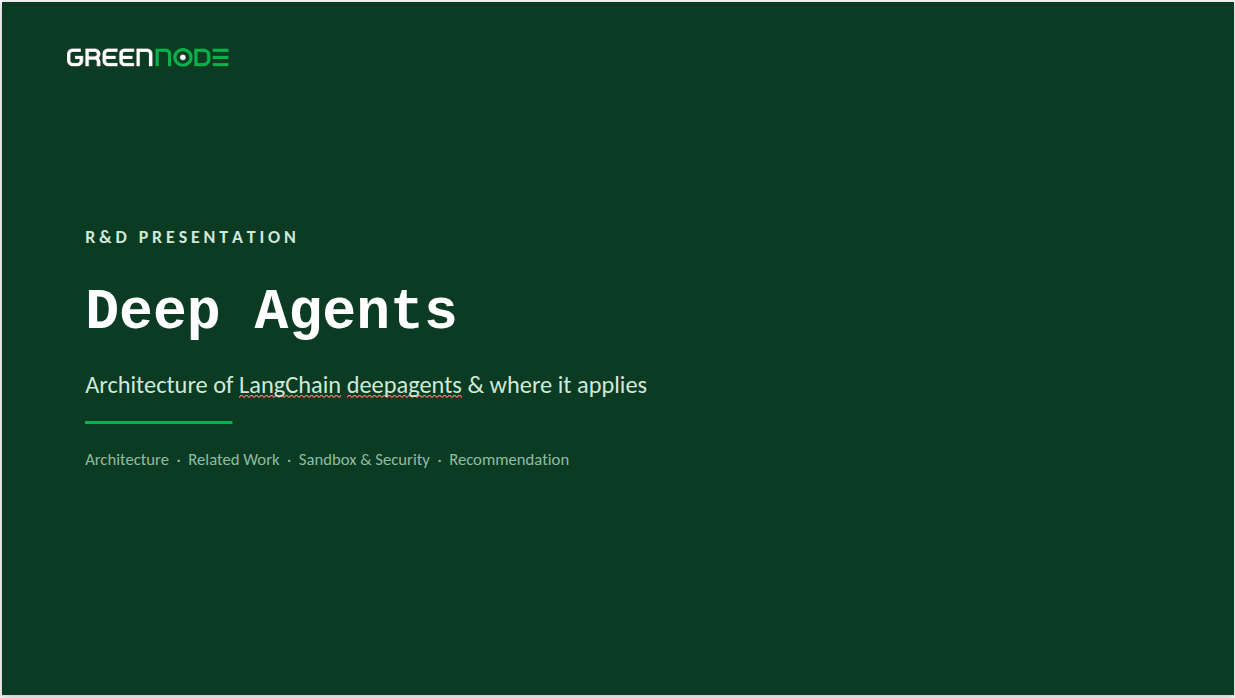
\includegraphics[width=\textwidth]{Images/page1.png}%
        \label{fig:deepagent_slide1}
    \end{minipage}
    \hfill
    \begin{minipage}[b]{0.49\textwidth}
        \centering
        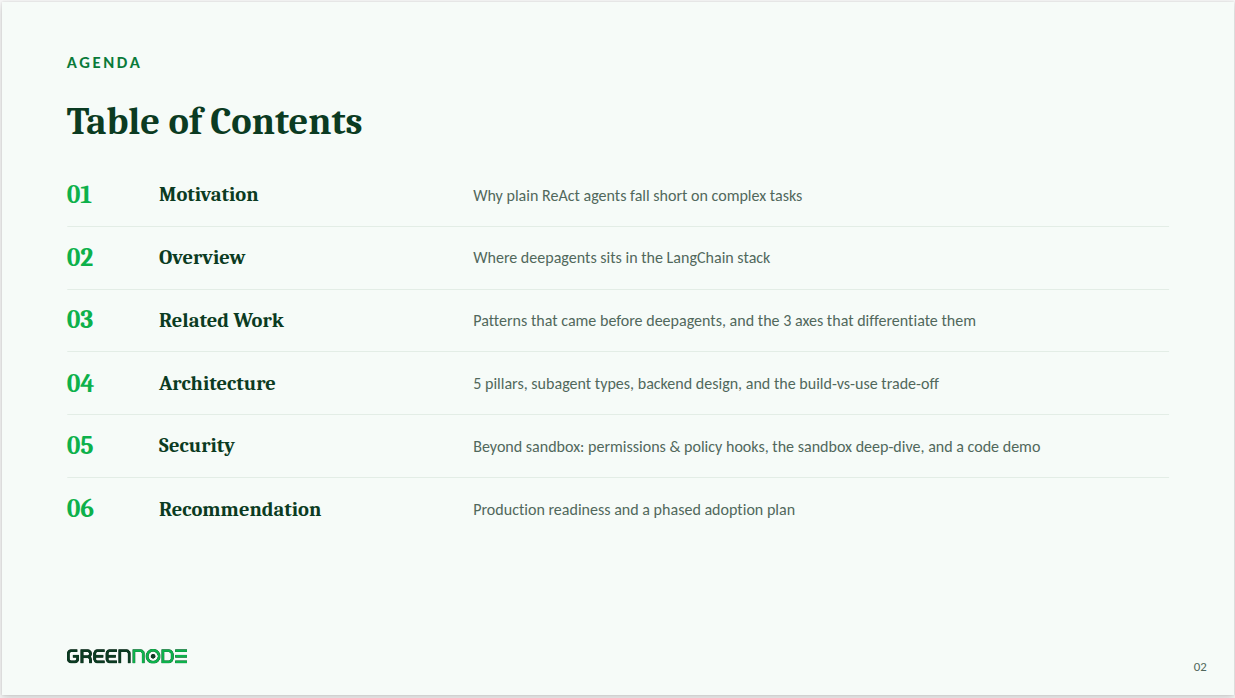
\includegraphics[width=\textwidth]{Images/page2.png}%
        \label{fig:deepagent_slide2}
    \end{minipage}
    \vspace{10pt}
    \caption{Deep Agent Seminar Slides}
    \end{figure}
\end{itemize}

\subsubsubsection*{Results / Knowledge Gained}

\begin{itemize}
    \item Delivered the Deep Agent seminar and communicated the proposed architectural direction to the team.
    \item Improved the team's understanding of the LangGraph scalability limitations and the role of a higher-level harness.
    \item Collected feedback to refine the migration plan for the final review.
\end{itemize}

\subsubsubsection{Week 12: Migration Plan and Line-Manager Review}

During Week 12, I consolidated the technical findings from the SRE Agent development and the Deep Agent seminar into a migration plan. I defined the proposed transition from the LangGraph-based implementation to a higher-level LangChain Deep Agent harness, clarified the migration priorities, and reviewed the recommendation with my line manager.

\subsubsubsection*{Task Description}

\begin{itemize}
    \item \textbf{Migration Plan Finalization}
    \begin{itemize}
        \item Defined migration phases for context management, memory, orchestration, tool calling, observability, governance, and controlled execution.
        \item Prioritized the components that should be migrated first to reduce LangGraph complexity without disrupting existing SRE Agent capabilities.
        \item Documented expected improvements in stability, scalability, maintainability, and future extensibility.
    \end{itemize}

    \item \textbf{Line-Manager Review}
    \begin{itemize}
        \item Presented the current SRE Agent architecture, LangGraph limitations, Deep Agent research, and proposed migration plan.
        \item Discussed technical risks, dependencies, implementation priorities, and future development requirements.
        \item Incorporated review feedback into the final documentation and handoff recommendations.
    \end{itemize}

    \item \textbf{Final Documentation and Handoff}
    \begin{itemize}
        \item Consolidated the internship results, architecture diagrams, research findings, and recommended next steps.
        \item Prepared final handoff material for continued development of the SRE Agent and its future harness migration.
    \end{itemize}
\end{itemize}

\subsubsubsection*{Results / Knowledge Gained}

\begin{itemize}
    \item Produced a reviewed migration plan from the LangGraph-based SRE Agent to a higher-level Deep Agent harness.
    \item Clarified technical priorities and risks for future SRE Agent development.
    \item Completed the final review and handoff with a concrete architectural direction.
\end{itemize}


\subsection{Knowledge and Skills Acquired}

Throughout this internship, I gradually developed both the theoretical understanding and the practical skills required to design, implement, evaluate, and improve AI-agent systems. My learning followed the same progression as the project itself: I began with agent foundations, applied them to the SRE Agent, added supporting execution and observability capabilities, and finally investigated a more scalable harness architecture. As a result, I was able to connect individual technologies to the practical requirements of a complete agent-development workflow.

\subsubsection{Agent Frameworks and LangGraph}

At the beginning of the internship, I studied the main concepts and development patterns used in agentic AI systems, including ReAct, reflection, self-critique, tool calling, state management, and execution loops. I then compared different agent-framework approaches and selected LangGraph for the initial prototype because it provided explicit control over workflow states, execution nodes, transitions, and tool integration.

Using this foundation, I first implemented a basic research and self-reflection agent and subsequently applied the same principles to build the SRE Agent. Through this process, I learned how to design agent state, define tool interfaces, connect reasoning with actions, handle tool results, and manage the transition from planning to execution, reflection, and final response generation. At the same time, the growing SRE Agent showed me that explicit graph-based orchestration can become increasingly difficult to extend when the number of states, tools, and execution requirements grows.

\subsubsection{Sandbox and Container Runtime}

Building on the SRE Agent workflow, I studied sandboxing as a supporting execution environment rather than as an independent project. In particular, I researched OpenSandbox and compared several container-runtime isolation approaches, including gVisor with \texttt{runsc}, Firecracker with \texttt{kata-fc}, and QEMU with \texttt{kata-qemu}.

To understand the practical trade-offs between these approaches, I considered isolation strength, startup latency, code-execution latency, memory footprint, and network throughput. In addition, I learned how Kubernetes pods, resource limits, timeout handling, output capture, and cleanup procedures can be used to control agent-related execution. Finally, I integrated the sandbox execution path with the SRE Agent in the staging environment and tested how agent tool invocation interacted with controlled execution.

\subsubsection{Observability with Jaeger}

After establishing the SRE Agent's core backend logic, I learned how Jaeger could be used to observe agent behavior in detail. I added tracing for LLM calls, tool invocations, state transitions, decision loops, reflection cycles, and execution latency.

These traces allowed me to examine the agent's internal execution rather than relying only on its final responses. Consequently, I learned how to identify slow execution steps, verify whether tools were invoked correctly, investigate errors, and analyze the behavior of individual decision loops. This experience strengthened my ability to debug and improve agent systems using observable execution evidence.

\subsubsection{Deep Agent Harness}

In the final phase, I investigated the LangChain Deep Agent harness after recognizing that the expanding LangGraph implementation was becoming difficult to scale and maintain. I studied how a higher-level harness could manage orchestration, context, memory, tool use, iteration control, timeout handling, state persistence, observability, permissions, human approval, and future multi-agent coordination.

I then compared the responsibilities implemented explicitly in the LangGraph-based SRE Agent with the capabilities offered by the Deep Agent harness. Although the proposed migration would change the orchestration layer, the existing SRE Agent capabilities could remain the functional core. Based on this comparison, I developed a migration direction in which the higher-level harness would manage orchestration and runtime concerns while preserving the agent's existing operational purpose.
\subsection{Deliverables}

During the internship, I produced several technical deliverables that together formed the foundation for the future development of GreenNode's internal SRE Agent. In particular, these deliverables combined the agent itself with the supporting execution, observability, documentation, and handoff materials.

\begin{figure}[H]
    \centering
    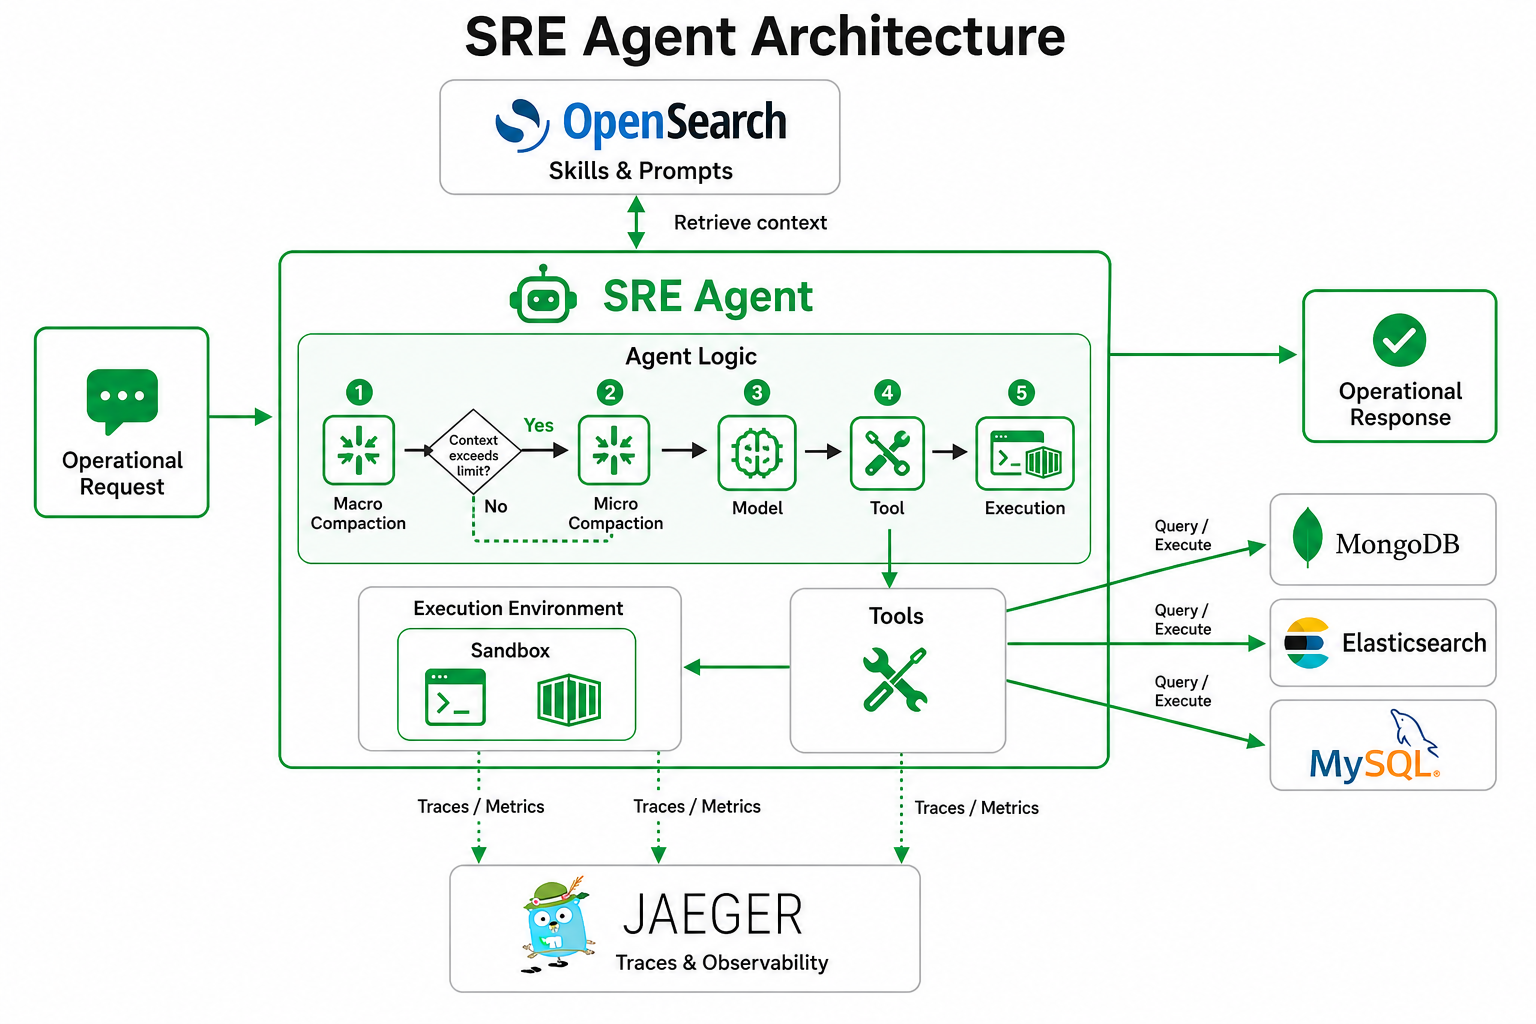
\includegraphics[width=\linewidth]{Images/full_arch.png}
    \caption{Complete SRE Agent Architecture and Supporting Components}
    \label{fig:full_architecture}
\end{figure}

\subsubsection{SRE Agent}

My main technical deliverable was an SRE Agent designed to support internal operational troubleshooting. I built the agent from the basic agent foundations developed during the first month of the internship. The agent can interpret an operational request, plan diagnostic actions, invoke the appropriate tools, manage execution state, evaluate tool results, and generate a structured response.

I also refined the agent's error-handling and execution flow so that diagnostic actions could be followed and analyzed more consistently. In addition, the Week 9 demonstration in Figure~\ref{fig:sre_agent_demo} presents the SRE-Agent workflow and its operational interface.

\subsubsection{Supporting Sandbox Execution Environment}

I integrated a sandbox execution path with the SRE Agent in the staging environment. In this way, the sandbox provided controlled execution for code-related or diagnostic actions while preserving the main SRE Agent workflow.

Before wiring, I conducted the benchmark of the sandbox execution path and compared the performance of different container runtimes. I also tested the sandbox's ability to handle timeouts, resource limits, output capture, and cleanup procedures. Finally, I verified that the SRE Agent could invoke tools through the sandbox and that the overall workflow remained functional and reliable.

\subsubsection{Agent Observability}

I added Jaeger-based observability to the SRE Agent. The instrumentation records important parts of the agent execution, including LLM calls, tool invocations, state transitions, decision loops, and execution latency.

Consequently, this observability layer made it possible to inspect agent behavior, analyze execution bottlenecks, verify tool interactions, and support future debugging and performance improvement.

\subsubsection{Architecture and Research Materials}

I prepared architecture diagrams and technical research materials describing the agent workflow, the SRE Agent architecture, the sandbox execution path, the observability connection, and the proposed Deep Agent harness direction.

I also produced a comparison of the current LangGraph implementation and the higher-level Deep Agent approach. Consequently, these materials were used to explain the current system, its scalability limitations, and the possible migration direction.

\subsubsection{Evaluation and Handoff Status}

I evaluated the agent using representative diagnostic flows and execution traces. During the evaluation, I considered task completion, response quality, tool performance, error handling, reflection behavior, and execution latency.

However, I did not record a final numerical task-success rate or a complete numerical latency benchmark during the internship. Therefore, I do not report fabricated performance values. Instead, the available evaluation evidence consists of functional demonstrations, representative workflow tests, Jaeger traces, observed execution behavior, and qualitative analysis of the agent's correctness and reliability.

At the end of the internship, the SRE Agent, its supporting sandbox execution path, and its Jaeger observability layer had been developed and evaluated in the staging environment. In addition, I completed the Deep Agent seminar, migration plan, architecture documentation, and handoff materials. Although the migration from the LangGraph implementation to the LangChain Deep Agent harness was not completed in production, it remained a clearly defined planned future direction.

\newpage
\section{Conclusion}
% \begin{itemize}
%     \item Kết thúc kỳ thực tập, SV thu nhận được những kỹ năng/ kiến thức gì?
    
%     \item Cảm nhận cá nhân: về DN, về chương trình thực tập?
%     \item SV ký và ghi rõ họ tên (chữ ký sống/ trực tiếp bằng bút màu xanh).

% \end{itemize}

During this three-month internship on AI Innovation for Internal Product Development, I strengthened my knowledge of large language models, ReAct and Harness agent frameworks, and supporting infrastructure such as Kubernetes. I also gained hands-on experience building the SRE Agent from the ground up, from the initial agent foundations through core logic, sandbox integration, and observability, while researching GreenNode's infrastructure and data sources along the way. This experience gave me a practical understanding of the full agent-development lifecycle, from theory and experimentation to production-oriented design.

I found GreenNode to be a supportive and innovative working environment. The guidance from my mentors, together with the opportunity to work with real systems and infrastructure, helped me improve both my technical and problem-solving skills. Overall, the internship deepened my interest in building stable, scalable, and valuable AI systems for real-world use.

\begin{flushright}
\begin{minipage}{0.4\textwidth}
  \rule{0.9\linewidth}{0.5pt}
  \centering
  \vspace{5pt}
  Student Signature\\
  
\includegraphics[width=0.4\linewidth]{Images/Signature_Phuoc.jpeg}\\
  Phạm Duy Tường Phước
\end{minipage}
\end{flushright}

\end{document}


